\section{Several modern programming languages and their designs}

We choose serval MPLs to analyze their designs systematically.
We give the definition for MPL, accordingly choose nine MPLs,
and explain the aspects of their designs to be analyzed.


%There is no uniform definition for MPL\@.
%Many researchers define it in different ways, such as finding
%connections between software engineering\cite{ModernProgrammingLanguagesSoftwareEnginerring}
%and the development of MPLs or elaborating
%around abstractions\cite{ModernProgrammingLanguagesAbstraction}.
%The above are correct in their respective fields,
%and here the definition is abstracted and extended to
%adapt to more domains.
%By studying the intersection of different definitions,
%a more general definition of MPLs derives.
%It is an obvious fact, that as the practice of
%programming languages continues to deepen, so does
%the definition of MPL. This is because PLT is a field
%where practice and theory go hand in hand.
%Although its definition is constantly changing, some
%core elements remain the same.
%Here are a few features of MPLs.

\subsection{Definition of modern programming language}

Researchers define MPL in different ways.
For example, some scholars define it from the perspective of software
engineering – as it develops, programming languages evolve into MPLs\cite{ModernProgrammingLanguagesSoftwareEnginerring}.
While others consider the key feature of MPL its abstraction\cite{ModernProgrammingLanguagesAbstraction}.
In fact, as the practical technology of programming languages progresses,
the definition of MPL will keep altering, because it is a combination
of both theory and practice.
However,although its definition keeps altering,
some core contents remain unchanged.
After studying multiple definitions given in the literature, we present a
more general description for MPL, which has the following features:

%\begin{enumerate}
%    \item Substance over form. It should provide descriptive grammatical structures, rather than hand-in-hand telling the machine what to do. This item emphasizes the abstraction of machine functions.
%    \item Semantic consistency. For similar grammatical structures, there should be similar grammatical functions.
%    \item Syntax bootstrapping. For non-core grammatical features, based on following semantic consistency, they should be composed of core grammatical features.
%    \item Paradigm convergence. Multiple programming paradigms should be provided without forcing users to use a particular programming paradigm.
%\end{enumerate}

\begin{enumerate}
    \item Substance over form. MPLs should emphasize what is important to the users and restrain what is not.
    \item Semantic consistency. For similar grammatical structures, there should be similar semantics.
    \item Syntax bootstrapping. For non-core grammars, following semantic consistency, they should be composed of core grammars.
    \item Paradigm convergence. Multiple programming paradigms should be provided without forcing users to use a particular one.
\end{enumerate}

\begin{table*}[htb]
    \caption{Features that a well-designed programming language should have}
    \label{tab:evaluate}
    \begin{center}
        \begin{tabular}{ccc}
            \toprule
            Evaluation Item & Meaning & Related Content \\
            \midrule
            Expressiveness &
            \makecell[l]{
                For abstract and complex business logic, programming \\
                languages can provide a concise way to describe it.
            }
            & Programming Paradigm, Type System \\
            \midrule
            Maintainability &
            \makecell[l]{
                After completing the business logic according to \\
                standard coding specifications, it is also easy to add new \\ features or
                fix bugs subsequently.
            }
            & Programming Paradigm, Type System \\
            \midrule
            Reliability &
            \makecell[l]{
                Non-crash under extreme conditions after completing \\
                business logic according to standard coding specifications.
            }
            & Programming Paradigm, Type System \\
            \midrule
            Performance &
            \makecell[l]{
                Deploying a software system written in this programming \\
                language takes up fewer hardware resources when running \\ on the target
                machine.
            }
            & Time Overhead, Memory Overhead \\
            \bottomrule
        \end{tabular}
    \end{center}
\end{table*}

\subsection{Selecting modern programming languages to be analyzed}

We select the MPLs to be analyzed based on the following considerations.
We first select the current most popular programming languages.
Next, there are many classification standards for programming languages.
For each standard, the selected programming languages should cover most of the categories.
Finally, we should focus on the new programming languages.
These programming languages have absorbed the advantages of past languages and
alleviated their inherent shortcomings.

According to the data of the IEEE spectrum,the top five popular programming
languages in 2021 are Python, Java, C, C ++, and JavaScript\cite{IEEETopProgrammingLanguages}.
Among them, C cannot be considered an MPL, due to its underlying syntax design.
We thus select the other four popular programming languages as our research objects.
It should be noted that, even though nowadays they are not exactly in line with the
features of MPL, they were the representative symbols of MPLs back when they
were initially developed.

%For the selection of programming language, the first thing is to pay attention to the most popular trend at the moment, so the selected programming language must cover the most commonly used. Secondly, there are many classification standards for programming languages. For each division standard, the selected programming language should cover most of the options. Then, it should focus on highlighting the new programming language with excellent design in recent years. These programming languages have absorbed the advantages of past programming languages and improved their inherent shortcomings. From these selected MPLs, we can see the development trend of application-oriented programming languages over the years.

According to the degree of popularity, we select five new-born MPLs -
Go, Swift, Dart, Rust, and Kotlin (where Swift and Dart are equally popular).
Coincidentally, these languages were also released in this order.
In addition, they all have similar type systems and support AOT compilation,
and although not all of them use garbage collection memory management,
they all move away from manual memory management.
These are all common features of MPLs in today’s application environment.

\begin{figure}[htbp]
    \centerline{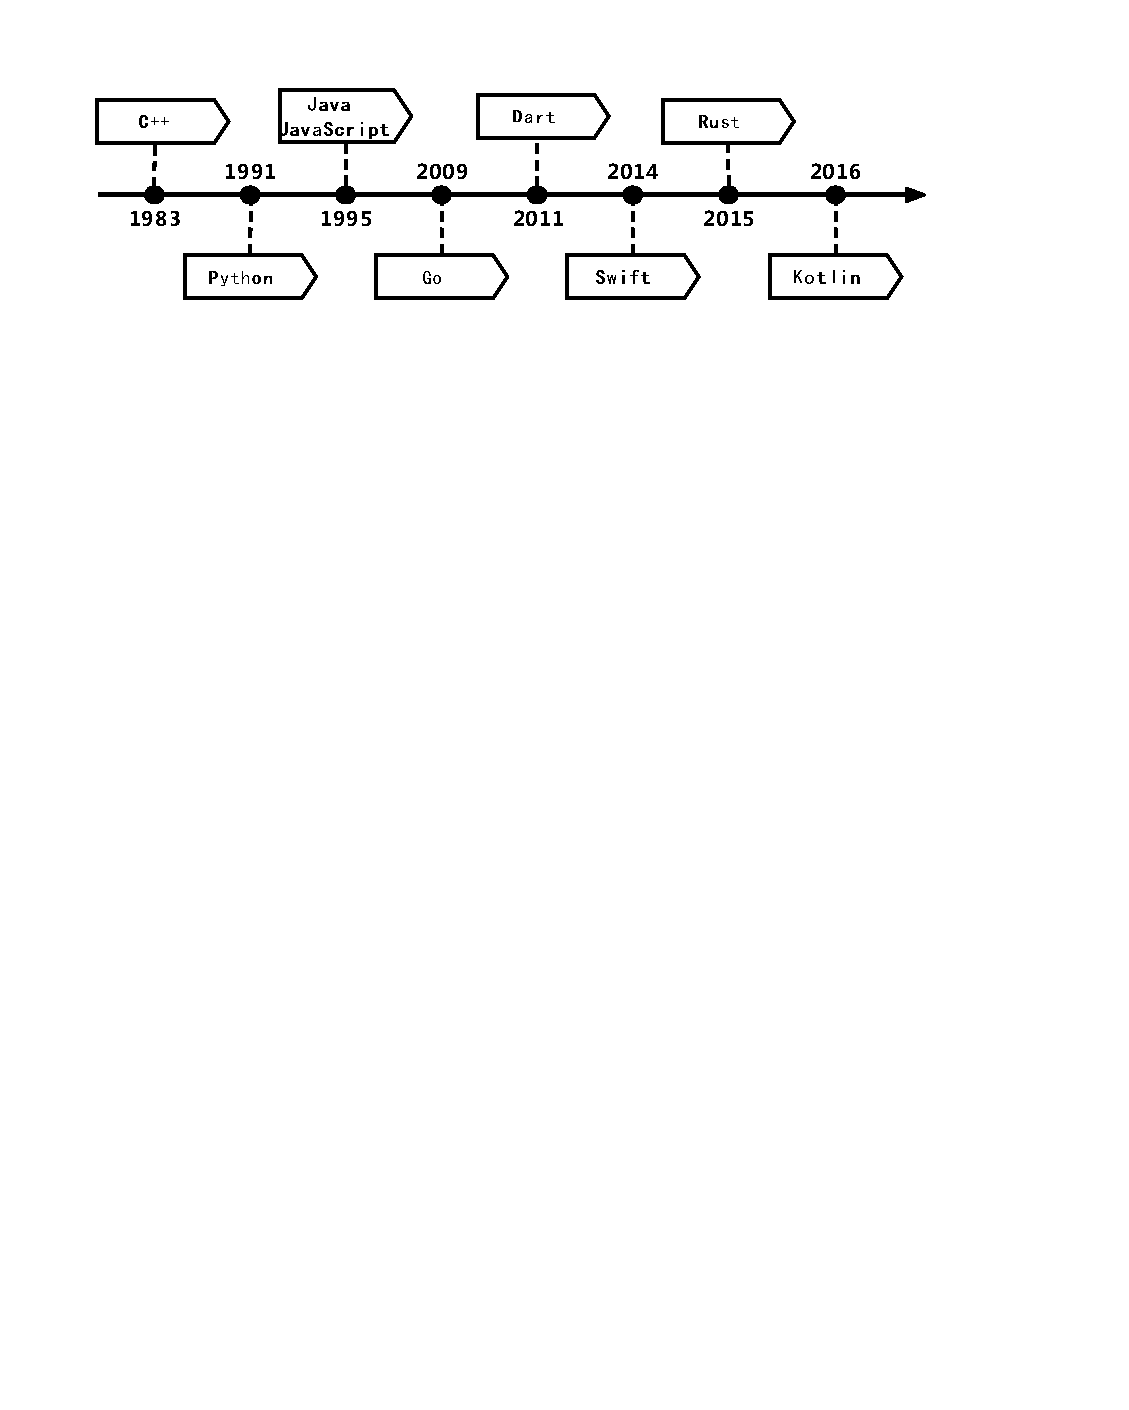
\includegraphics[scale=0.6]{figures/timeline}}
    \caption{Timeline of several MPLs}
    \label{fig:timeline}
\end{figure}


The timeline of the birth of the nine selected MPLs is shown in Figure~\ref{fig:timeline}.

%According to the data of the IEEE spectrum\cite{IEEETopProgrammingLanguages},
%the top five most popular programming languages in 2021 are Python, Java, C, C ++, and JavaScript. An exception case is C, which provides low-level access to computer systems. To be precise, the syntax design of the C language does not conform to any of the features of MPL. And for the four remaining popular programming languages mentioned above, they are still helpful even though they are not exactly in line with the features of MPL. In the era when these languages were first created, they emerged as representatives of MPLs. Therefore these four past programming languages are compared with the emerging MPLs.


%Based on the above-mentioned MPL features,
%several programming languages were selected and arranged
%in order of popularity\cite{IEEETopProgrammingLanguages},
%resulting in Go, Swift, Dart, Rust and Kotlin (where Swift and Dart are equally popular).
%Coincidentally, these languages are also released in this order sequentially, see Figure\ref{fig:timeline}.
%In addition, all of these languages have similar type systems and all support AOT compilation, and although not all use garbage collection memory management, they all move away from manual memory management.
%These are all common features of MPLs in today's application environment, as we can see from Table\ref{tab:selected-languages}.

\subsection{Criteria to evaluate the design of programming languages}


%We think there are two main aspects that determine whether a language is useful or not.
%One aspect is its syntactic design.
%For complex business logic, programming languages are required to provide
%strong expressiveness, i.e., isolate underlying implementations
%that are not related to the business logic to accommodate rapid changes.
%Programming languages are also needed to provide solutions for
%checking the correctness and reliability of programs.
%Another aspect is performance, where programming languages are
%always expected to have a low memory overhead and time overhead,
%relying heavily on compile-time (native languages) and run-time
%(virtual machine languages) optimizations.
%See Table\ref{tab:evaluate}.


We assess the designs of these MPLs from an application-oriented point of view.
In other words, we evaluate whether a language design is “practical”.
There are mainly two aspects that determine whether a language is practical or not.
One is its syntactic design.
For complex business logic, programming languages are required to provide strong expressiveness,
i.e., isolate underlying implementations that are not related to the business logic to
accommodate rapid changes.
Programming languages also need to provide solutions for correctness checking and program reliability.
Another aspect is performance, where programming languages are always expected to have
a low memory overhead and time overhead, which rely heavily on compile-time (native languages)
and run-time (virtual machine languages) optimizations.
Specifically, the evaluation criteria of this paper are presented in Table~\ref{tab:evaluate}.
For expressiveness, maintainability, and reliability of a language, we analyze them
by programming paradigm or type system;
for Performance of a language, we analyze it by time overhead and memory overhead.
And the introduction of the nine selected MPLs about their programming paradigm,
type system, compilation mode and memory model are shown in Table~\ref{tab:selected-languages}.

\begin{table*}[ht]
    \caption{Several modern programming languages}
    \label{tab:selected-languages}
    \begin{center}
        \begin{tabular}{ccccccc}
            \toprule
            Language & Programming Paradigm & Type System & Compilation Mode & Memory Model &
            Release Date & Application Scenarios \\
            \midrule
            Python & Multi-paradigm & Dynamically, Strongly & JIT & GC & 1991 & Web,
            Enterprise, Embedded \\
            Java & Multi-paradigm & Statically, Strongly & AOT & GC & 1995 & Web,
            Mobile, Enterprise \\
            C++ & Multi-paradigm & Statically, Weakly & AOT & Manual & 1983 & Mobile,
            Enterprise, Embedded \\
            JavaScript & Multi-paradigm & Untyped & JIT & GC & 1995 &
            Web \\
            Go & Multi-paradigm & Statically, Strongly & AOT & GC & 2009 & Web,
            Enterprise \\
            Swift & Multi-paradigm & Statically, Strongly & AOT & ARC & 2014 &
            Mobile, Enterprise \\
            Dart & Multi-paradigm & Statically, Strongly & AOT\&JIT & GC & 2011 &
            Web, Mobile \\
            Rust & Multi-paradigm & Statically, Strongly & AOT & Ownership & 2015 &
            Web, Enterprise, Embedded \\
            Kotlin & Multi-paradigm & Statically, Strongly & AOT\&JIT & GC & 2016 &
            Web, Mobile \\
            \bottomrule
        \end{tabular}
    \end{center}
\end{table*}

%In practice, however, programming language design cannot be accurately quantified.
%The reason for this is twofold.
%The first is that certain criteria for evaluation are not quantitative.
%For expressiveness and reliability, both are abstract descriptions,
%and they have uncountable kinds of cases in practice.
%If one wants to analyze them quantitatively, then one must restrict the analysis to
%certain specific application scenarios.
%The second is that the evaluation criteria are not sufficient.
%Some evaluation criteria that are difficult to measure, such as response time in a
%real-time system, are dropped here for structural completeness.
%For programming languages with garbage collectors, the performance loss from garbage collection is not negligible. In particular, JVM-based programming languages have the problem of "Stop the World" when garbage collection is performed, which affects the performance of the programming language. However, this is not considered for the sake of simplicity.


It should be emphasized that programming language design cannot be fully
evaluated by quantitative analysis.
For expressiveness and reliability, which are descriptions for abstract concepts,
although quantitative analysis is possible, it is usually limited to a certain
application environment, which does not have much significance.
Some other performances are difficult to measure, such as response time in real-time systems.
Additionally, for programming languages with garbage collectors, the performance
loss from garbage collection is not negligible.
In particular, JVM-based programming languages have the problem of "Stop the World"
when garbage collection is performed\cite{gidra2013study},
which affects the performance of the programming language.
Such features are not considered in this paper.